\documentclass[b5paper]{article}
% Add "final" option in the article to remove todo
\usepackage[tight,common_math_textnormal,todonotes,math_base_note,math_simple]{gatmeo}
\usepackage{tikz-cd}

\title{\bf{
Hypertoric Varieties Arose from Graphs
}}

\newcommand{\noskipline}{\vspace{-1.5em}}

\renewcommand{\epsilon}{\varepsilon}
\renewcommand{\phi}{\varphi}
\newcommand{\NN}{\mathbb{N}}
\newcommand{\ZZ}{\mathbb{Z}}
\tikzcdset{
    cells={font=\everymath\expandafter{\the\everymath\displaystyle}},
}

% Hypertoric Variety
\newcommand{\MM}{\mathcal{M}}
\newcommandx*\Mper[1][1=\Gamma]{\mathcal{M}^{\mathrm{per}}(#1)}
\newcommandx*\Mperchar[2][2=\Gamma]{\mathcal{M}^{\mathrm{per}}_{#1}(#2)}
\newcommandx*\Hper[1][1=\Gamma]{\mathcal{A}^{\mathrm{per}}(#1)}
\newcommandx*\Hperchar[2][2=\Gamma]{\mathcal{A}^{\mathrm{per}}_{#1}(#2)}
\newcommandx*\Rper[2][1=\bullet, 2=\Gamma]{\mathcal{R}_{\mathrm{per}}^{#1}(#2)}
\newcommandx*\SRper[2][1=\bullet, 2=\Gamma]{\mathcal{SR}_{\mathrm{per}}^{#1}(#2)}
\newcommandx*\Mfin[1][1=\Gamma]{\mathcal{M}(#1)}
\newcommandx*\Mfinchar[2][2=\Gamma]{\mathcal{M}_{#1}(#2)}
\newcommandx*\Hfinchar[2][2=\Gamma]{\mathcal{A}_{#1}(#2)}
\newcommandx*\Hfin[1][1=\Gamma]{\mathcal{A}(#1)}
\newcommandx*\Rfin[2][1=\bullet, 2=\Gamma]{\mathcal{R}^{#1}(#2)}
\newcommandx*\SR[2][1=\bullet, 2=\Gamma]{\mathcal{SR}^{#1}(#2)}
\newcommandx*\Mmul[1][1=\Gamma]{\mathcal{M}^{\mathrm{mul}}(#1)}
\newcommandx*\idealIper[1][1=\Gamma]{I_{\mathrm{per}}(#1)}
\newcommandx*\idealI[1][1=\Gamma]{I(#1)}
\newcommand{\opendisc}{\mathbb{D}}
\newcommandx*\Betti[1][1=\Gamma]{\mathfrak{B}(#1)}
\newcommandx*\Dolbeault[1][1=\Gamma]{\mathfrak{D}(#1)}

% Core and Toric
\newcommandx*\corefin[1][1=\Gamma]{\mathcal{L}(#1)}
\newcommandx*\coreper[1][1=\Gamma]{\mathcal{L}^{\mathrm{per}}(#1)}
\newcommandx*\toricP[1][1=P]{\mathcal{X}(#1)}
\newcommandx*\fixptP[1][1=B]{P_{#1}}
\newcommandx*\toricB[1][1=B]{\mathcal{X}(#1)}

% Complex
% Group Cohomology Complex
\newcommand{\pGC}{\mathfrak{C}} 
\newcommandx*\GC[3][1=\bullet,2=\bullet,3=\Gamma]{\mathfrak{C}^{#1,#2}(#3)} % Our complex: Group Cohomology
\newcommand{\dGC}{\delta} % Our complex: Group Cohomology
\newcommand{\dGCbar}{\bar{\delta}} % Our complex: Group Cohomology
\newcommand{\fGC}{\phi}
\newcommand{\gGC}{\psi}
\newcommand{\hGC}{\eta}
%--- Group Cohomology Complex with e
\newcommandx*\GCe[4][1=\bullet,2=\bullet,3=\Gamma,4=e]{\mathfrak{C}^{#1,#2}(#3,#4)}
\newcommand{\dGCe}{\delta_e}
\newcommand{\fGCe}{\mathfrak{f}}
\newcommand{\gGCe}{\mathfrak{g}}
\newcommand{\hGCe}{\mathfrak{h}}
%--- CKS
\newcommandx*\GCS[2][1=\bullet,2={\Gamma, S}]{\mathfrak{D}^{#1}(#2)}
\newcommandx*\dGCS[1][1=S]{\dGC_{#1}}
\newcommandx*\fGCS[1][1=S]{\fGC_{#1}}
\newcommandx*\gGCS[1][1=S]{\gGC_{#1}}
\newcommandx*\hGCS[1][1=S]{\hGC_{#1}}
\newcommandx*\CKS[4][1=\bullet,2=\bullet,3=\bullet,4=\Gamma]{\mathfrak{C}^{#1,#2,#3}(#4)} % CKS
\newcommandx*\grCKS[4][1=\bullet,2=\bullet,3=\bullet,4=\Gamma]{I^{#1, #2}\mathfrak{C}^{#3}(#4)} % CKS
\newcommandx*\CKSdiffgrading[3][1=\bullet,2=\bullet,3=\Gamma]{\mathfrak{C}'^{#1,#2}(#3)} % CKS
\newcommand{\dCKS}{d} %CKS Complex
\newcommand{\fCKS}{f}
\newcommand{\gCKS}{g}
\newcommand{\hCKS}{h}
\newcommandx*\HT[3][1=\bullet,2=\bullet,3=\Gamma]{\mathfrak{K}_{\mathrm{per}}^{#1, #2}(#3)}
\newcommandx*\grHT[3][1=\bullet,2=\bullet,3=\Gamma]{I^{#1}\mathfrak{K}_{\mathrm{per}}^{#2}(#3)}
\newcommand{\dHT}{\dCKS_{\mathrm{per}}}
\newcommandx*\HTalt[2][1=\bullet,2=\Gamma]{\tilde{\mathfrak{K}}^{#1}(#2)}
\newcommand{\dHTalt}{\tilde{\dCKS}_{\mathrm{per}}}
\newcommand{\fHT}{\fCKS_{\mathrm{per}}}
\newcommand{\gHT}{\gCKS_{\mathrm{per}}}
\newcommand{\hHT}{\hCKS_{\mathrm{per}}}
\newcommandx*\HTfin[3][1=\bullet,2=\bullet,3=\Gamma]{\mathfrak{K}^{#1, #2}(#3)}
\newcommandx*\grHTfin[3][1=\bullet,2=\bullet,3=\Gamma]{I^{#1}\mathfrak{K}^{#2}(#3)}
\newcommand{\dHTfin}{\dCKS}
\newcommand{\fHTfin}{\fCKS}
\newcommand{\gHTfin}{\gCKS}
\newcommand{\hHTfin}{\hCKS}
\newcommandx*\CPX[3][1=\bullet,2=\bullet,3=\Gamma]{\mathfrak{D}^{#1,#2}(#3)} % Intermediate complex
\newcommandx*\euler[3][3=\Gamma]{\eta^{#1, #2}(#3)}

% Graph and Matroids
\newcommandx*\Tutte[2][1=\Gamma]{T(#1;\, #2)}
\newcommandx*\hpoly[2][1=\Gamma]{h(#1;\, #2)}
\newcommandx*\HTutte[2][1=\Gamma]{H(#1;\, #2)}
\newcommandx*\seqn[1][1=n]{[-#1,#1]}
\newcommand{\loopgraph}{{\bigcirc\!\!\bullet}}
\newcommand{\bridgegraph}{{\bullet\mspace{-7mu}-\mspace{-7mu}\bullet}}
\newcommand{\supnorm}[1]{\| #1 \|_{\infty}} 

\newcommand{\del}{\setminus}
\newcommand{\con}{\mathbin{/}}
\newcommand{\Gammaper}{\Gamma_{\mathrm{per}}}
\newcommandx*\tree[2][2=\Gamma]{\mathcal{T}_{#2}(#1)}
\newcommandx*\treefunction[1][1=\Gamma]{\mathcal{T}_{#1}}
\newcommandx*\cotreefunction[1][1=\Gamma]{\mathcal{T}_{#1}^*}
\newcommandx*\cotree[2][2=\Gamma]{\mathcal{T}_{#2}^*(#1)}
\newcommandx*\face[2][1=\bullet,2=\Gamma]{F_{#1}(#2)}
\newcommandx*\faceshelling[3][2=\bullet,3=\Gamma]{F_{#2}^{(#1)}(#3)}
\newcommandx*\faceper[2][1=\bullet,2=\Gamma]{F^{\mathrm{per}}_{#1}(#2)}
\newcommandx*\pair[3][3=\Gamma]{\langle #1, #2 \rangle_{#3}}
\newcommandx*\cotreein[2][2=\Gamma]{\mathcal{D}_{#2}(#1)}
\newcommandx*\cotreeinper[2][2=\Gamma]{\mathcal{D}^\per_{#2}(#1)}
\newcommandx*\cotreeinfunction[1][1=\Gamma]{\mathcal{D}_{#1}}
\newcommandx*\externalactivity[2][2=\Gamma]{EA_{#2}(#1)}
\newcommandx*\internalactivity[2][2=\Gamma]{IA_{#2}(#1)}
\newcommand{\intp}[1]{\iota_{#1}} % interior product
\newcommandx*\fundcycle[2][2=\Gamma]{C_{#2}(#1)}
\newcommandx*\fundcyclewithtree[3][2=\Gamma,3=T]{C_{#2}(#3,#1)}
\newcommandx*\basis[2][1=\bullet,2=\Gamma]{\mathcal{B}_{#1}(#2)}
\newcommandx*\basisper[2][1=\bullet,2=\Gamma]{\mathcal{B}^\per_{#1}(#2)}

\newcommandx*\SE[3][1=,3=]{
  \ifstrempty{#3}
  {\ifstrempty{#1}{E^\bullet_{#2}}{#1_{#2}}}
  {\ifstrempty{#1}{E_{#2}(#3)}{#1_{#2}}}
}
\newcommandx*\HMGZ[2][1=\Gamma,2=\bullet]{H^{#2}(\MM(#1),\mathbb{Z})}
\newcommand{\hCCC}{\hat{\mathfrak{C}}}

\newcommand{\per}{\mathrm{per}}

% Math Operations
\newcommand{\HH}{\mathrm{H}}
\newcommandx*\Ext[1][1=\bullet]{\bigwedge\nolimits^{#1}}
\newcommandx*\Sym[1][1=\bullet]{\mathrm{Sym}^{#1}}
\newcommand{\sgn}{\mathrm{sgn}}
\newcommand{\coker}{\operatorname{coker}}
\renewcommand{\im}{\operatorname{Im}}
\newcommand{\supp}{\mathrm{supp}}
\newcommand{\Hom}{\mathrm{Hom}}

% Group Cohomology
\newcommand{\invar}[1]{\Gamma_{#1}}
\newcommandx*\Rder[1][1=\bullet]{R^{#1}}
\newcommandx*\totRder[1][1=\bullet]{\mathbb{R}^{#1}}

% Homotopy Equivalence
\newcommand{\choice}[1]{[#1]} % choice for HTfin equiv
\newcommandx*\intord[2][2=S]{[#2]^{#1}} % integration order for GCS equiv
\newcommandx*\hyppl[2][2=S]{\alpha^{#2}_{#1}} % hyperplane for GCS equiv

\makeatletter
\newcommand{\GIT}[1][\@nil]{%
  \def\tmp{#1}%
  \ifx\tmp\@nnil
    /\!\!/%
  \else
    /\!\!/_{\! #1}%
  \fi
}
\newcommand{\HQ}[1][\@nil]{%
  \def\tmp{#1}%
  \ifx\tmp\@nnil
    /\!\!/\!\!/\!\!/%
  \else
    /\!\!/\!\!/\!\!/_{\! #1}%
  \fi
}
\makeatother

\newcommand{\Diff}{\mathrm{Diff}}
\newcommand{\Sympl}{\mathrm{Sympl}}
\newcommand{\acton}{\curvearrowright}
\newcommand{\smth}{C^\infty}
\newcommand{\df}{\Omega}
\newcommand{\vf}{\mathrm{Vec}}
\newcommand{\svf}{\mathrm{Vec}_\mathrm{sym}}
\newcommand{\hvf}{\mathrm{Vec}_\mathrm{ham}}
\newcommand{\ind}[1]{#1^\#}
\newcommand{\lied}[1]{\mathcal{L}_{#1}}
\newcommand{\intd}[1]{\iota_{#1}}
\newcommand{\Proj}{\textnormal{Proj }}
\newcommand{\Spec}{\textnormal{Spec }}
\newcommand{\sstab}{\mathrm{ss}}
\newcommand{\stab}{\mathrm{s}}

\begin{document}
\maketitle
\vspace{-3.5em}
%\input{abstract}

\thispagestyle{empty}
\tableofcontents
\listoftodos

\section{Symplectic Reduction for Toric Varieties}

\subsection{Symplectic Reduction for Hamiltonian Action}

Consider a Lie group $G$ acting on a manifold $M$. For $X\in\mathfrak{g}$, denote $\ind{X}$ the induced vector field on $M$. If we assume $M$ is symplectic and $G$ acts symplectically, i.e. $G$ preserve symplectic form, the action is Hamiltonian if there also exists a moment map $\mu : M \to \mathfrak{g}^*$ such that
\begin{enumerate}
    \item $\mu$ is $G$-equivariant where $G$ acts on $\mathfrak{g}^*$ by the coadjoint action, and
    \item for all $X \in \mathfrak{g}$, considered as $X : \mathfrak{g}^* \to \mathbb{R}$, $d(X \circ \mu) = \intd{\ind{X}}\omega$.
\end{enumerate}
If $G$ is abelian, then any shift $\mu+\alpha$, $\alpha\in\mathfrak{g}^*$, is also a moment map.

\begin{example}[exp:Cn_moment]{$\mathbb{T}_\mathbb{R}^n \acton \mathbb{C}^n$}
    Consider the real torus $\mathbb{T}_\mathbb{R}^n=(S^1)^n$ acting on $\mathbb{C}^n$ by rotating each coordinate. There is a canonical real symplectic form on $\mathbb{C}^n$ given by $\omega_\mathbb{R}=\sum_jdx_j\wedge dy_j$. Let $X_i\in\mathfrak{t}_\mathbb{R}^n$ be a standard basis vector, 
    the induced vector field $\ind{X_i}$ is given by
    \begin{align*}
        (\ind{X_i})_z &= \frac{d}{dt} [e^{2\pi it} z_i]_{t=0}
        = \frac{d}{dt} [(\cos(2\pi t) x_i - \sin(2\pi t) y_i,\sin(2\pi t)x_i + \cos(2\pi t)y_i)]_{t=0} \\
        &= (0, \dots, -2\pi y_i, \dots, 0, 0, \dots, 2\pi x_i, \dots, 0) = -2\pi y_i \left.\frac{\partial}{\partial x_i}\right|_z + 2\pi x_i \left.\frac{\partial}{\partial y_i}\right|_z.\\
        \intd{\ind{X_i}}\omega_\mathbb{R} &= \biggl(\sum_j dx_j \wedge dy_j\biggr)\left(-2\pi y_i \frac{\partial}{\partial x_i} + 2\pi x_i \frac{\partial}{\partial y_i}\right) = 
        = -2\pi (x_i \, dx_i + y_i \, dy_i).
    \end{align*}
    Thus, $\intd{\ind{X_i}}\omega_\mathbb{R} = d(-\pi(x_i^2 + y_i^2)) = d(-\pi|z_i|^2)$. Note that $X_i : (\mathfrak{t}^n)^* \to \mathbb{R}$ is regarded as the $i$th coordinate map. It follows that $\mu(z_1, \dots, z_n) = (-\pi|z_1|^2, \dots, -\pi|z_n|^2)$ is a choice of moment map.
\end{example}

It is easy to check that $\mu^{-1}(\xi) \subseteq M$ for any $\xi$ in the center of $\mathfrak{g^*}$ is $G$-invariant. Choose $\xi=0$, we define $M\GIT G=\mu^{-1}(0)\GIT G$ to be the symplectic reduction of $M$ by $G$ if $G$ acts on $\mu^{-1}(0)$ is free. In particular, if $G$ is abelian, we can do the reduction at different moment map level $\mu^{-1}(\xi)$.

\begin{theorem}{Marsden-Weinstein-Meyer Theorem}
    Assume that the restricted action $G $ on $ \mu^{-1}(0)$ is free. Let $\iota:\mu^{-1}(0)\rightarrow M$. Then,
    \begin{enumerate}
        \item $M \GIT G$ is a smooth manifold and $\pi:\mu^{-1}(0) \to M \GIT G$ is a principal bundle, and
        \item there is a symplectic form $\omega_{\mathrm{red}}$ on $M \GIT G$ satisfying $\iota^*\omega = \pi^*\omega_{\mathrm{red}}$.
    \end{enumerate}
\end{theorem}

\subsection{Symplectic Toric Manifold}

We define a symplectic toric manifold to be a compact connected $2n$-dimensional symplectic manifold $M$ with an effective real $n$-dimensional torus Hamiltonian action $T$, i.e. $T \to \Sympl(M)$ is injective.
We will see later that such spaces can be described using Delzant Polytopes, which correspond to complex $n$-dimensional connected projective toric varieties.

Let $\Delta \subseteq (\mathbb{R}^d)^*$ be a rational convex polytope with $n$ facets.
Such a polytope is said to be
\begin{itemize}
    \item \vocab{simple} if there are $d$ edges meeting at each vertex,
    \item \vocab{unimodular} if for all vertex $x$, there exist $v_1, \dots, v_n \in \mathbb{Z}^d$ that spans the $d$ edges such that $(v_1, \dots, v_d)$ forms a $\mathbb{Z}$-basis of $\mathbb{Z}^d$, and
    \item \vocab{Delzant} if it is rational, simple, and unimodular.
\end{itemize}
If we describe $\Delta$ as the intersection of $n$ affine hyperplanes, i.e. there exists normal vectors $a_i\in \mathbb{Z}^d$ and shifts $r_i\in\mathbb{R}$ such that 
\begin{equation*}
    \Delta = \{ x \in (\mathbb{R}^d)^* \mid \langle x, a_i \rangle \leq \theta_i \  \forall 1 \leq i \leq n \},
\end{equation*}
we can translate the above terminology: a hyperplane arrangement is said to be
\begin{itemize}
    \item \vocab{simple} if every $k$ hyperplanes with non-empty intersection intersect at codimension $k$;
    \item \vocab{unimodular} if every collection of $d$ independent vectors in $\{a_i\}$ forms a $\mathbb{Z}$-basis of $\mathbb{Z}^d$.
\end{itemize}
Let $\pi:\mathbb{Z}^n\rightarrow \mathbb{Z}^d$ be the $\mathbb{Z}$-linear map which sends the $i$-th basis vector to $a_i$. Unimodularity implies $\pi$ is surjective. Let $\mathbb{Z}^k$ be the kernel of $\pi$ where $k=n-d$, we have the following exact sequence:
\begin{equation}
  \label{eq:exact_seq_Z}
  \begin{tikzcd}[row sep=small]
    1 \arrow[r] & \mathbb{Z}^k \arrow[r, "\iota"] & \mathbb{Z}^n \arrow[r, "\pi"] & \mathbb{Z}^d \arrow[r] & 1.
  \end{tikzcd}
\end{equation}

Unimodularity also implies that the maximal minors of the matrix $\left[a_1|\dots|a_n\right]$ for $\pi$ are $0,\pm1$. In fact, one can check that the RREF of $\left[a_1|\dots|a_n\right]$ is totally unimodular, i.e. all minors are $0,\pm1$.

\begin{theorem}{}
  There is a one-to-one correspondence between Delzant polytopes and symplectic toric manifolds $(M, \omega, \mathbb{T}^d, \mu)$. In particular, $\im(\mu) \subseteq (\mathbb{R}^d)^*$ is a Delzant polytope. 
  \begin{proof}
    With the notation above, we claim that with a Delzant polytope $\Delta$, we can associate a symplectic toric manifold $M=\mathbb{C}^n \GIT \mathbb{T}^k$.
    \Cref{eq:exact_seq_Z} induces the following exact sequence of tori and lie algebras:
    \begin{equation*}
      \begin{tikzcd}[row sep=small]
        1 \arrow[r] & \mathbb{T}^k \arrow[r, "\iota"] & \mathbb{T}^n \arrow[r, "\pi"] & \mathbb{T}^d \arrow[r] & 1 \\
        0  & (\mathfrak{t}^k)^* \arrow[l] & (\mathfrak{t}^n)^* \arrow[l, "\iota^*"] & (\mathfrak{t}^d)^* \arrow[l, "\pi^*"] & 0\arrow[l].
      \end{tikzcd}
    \end{equation*}
    Consider the standard action $\mathbb{T}^n $ on $\mathbb{C}^n$ with moment map (\Cref{exp:Cn_moment}) $\mu : \mathbb{C}^n \to (\mathfrak{t}^n)^*$,
    \begin{equation*}
      \mu(z_1, \dots, z_n) = (-\pi|z_1|^2 + \theta_1, \dots, -\pi|z_n|^2 + \theta_n).
    \end{equation*}
    The inclusion $\iota$ induces an action $\mathbb{T}^k$ on $\mathbb{C}^n$, with moment map given by the composite $\iota^* \circ \mu : \mathbb{C}^n \to (\mathfrak{t}^k)^*$. This allows us to define the symplectic reduction $M = \mathbb{C}^n \GIT \mathbb{T}^k$. 
    \begin{itemize}
      \item $Z:=(\iota^*\circ \mu)^{-1}(0)=\mu^{-1}(\pi^*(\Delta))$ is compact: Consider $\pi^*:(\mathfrak{t}^d)^*\rightarrow (\mathfrak{t}^n)^*$ as the transpose of $\pi$. $\im(\pi^*)=\ker(\iota^*)\subseteq (\mathfrak{t}^n)^*$ is a $d$-dimension linear subspace cut out by the equation of $\iota^*$. Recall $\Delta$ is the intersection of half space $\CB{x\in (\mathfrak{t}^d)^*\mid \AB{x,\pi(e_i)}\leq \theta_i}$. $\pi^*(\Delta)\subseteq \im(\pi^*)$ then equals the intersection of half space $\CB{x\in \im(\pi^*)\subseteq (\mathfrak{t}^n)^*\mid \AB{x,e_i}\leq \theta_i}$. Hence 
        \[
          (\iota^*\circ \mu)^{-1}(0)=\mu^{-1}(\ker(\iota^*))=\mu^{-1}(\im(\pi^*))=\mu^{-1}(\pi^*(\Delta))
        \]
        is compact as $\mu$ is proper.
      \item $T^k$ acts freely on $Z$: For $z\in Z$, let $I_z=\CB{i\mid z_i=0}$. The stablelizer 
        \[
          T^n_z=\CB{t\in T^n\mid t_i=1\textnormal{ if }i\notin I_z}\simeq T^{I_z}.
        \]
        Recall $\mu_i(z)=-\pi|z_i|^2+\theta_i$, $z_i=0$ iff $\AB{\mu(z),e_i}=\theta_i$ iff $\AB{x,\pi(e_i)}=\theta_i$ for some $x\in \Delta$. Hence $I_z$ is the set of hyperplanes where $\mu(z)$ lies on. In particular, $|I_z|\leq d$. Since $\CB{\pi(e_i)\mid i\in I_z}$ is linearly independent, $\pi:T^n_z\rightarrow T^d$ is injective. Hence $T^k$ acts freely on $Z$.
    \item Moment polytope of $M$ is $\Delta$: The $T^d$ fix points of $M$ by the above discussion is hence the vertices of $\Delta$. We omit the remaining of the proof.
    \end{itemize}
  \end{proof}
\end{theorem}

In fact, the polytope $\pi^*(\Delta)=\ker(\iota^*)\cap \CB{x_i\leq \theta_i}$ can be shifted to the intersection of $\bigcap \CB{x_i\leq 0}$ with a affine subspace $\im(\pi^*-\theta)=\ker(\iota^*+\iota^*(\theta))$. Hence in order to describe $\pi^*(\Delta)$, it is suffice to specify an element $\iota^*(\theta)\in (\mathfrak{t}^k)^*$. The moment map also depends only on $\iota^*(\theta)$ instead of $\theta$. In other words, to define a symplectic toric variety, we can choose the standard moment map $\mu_\textnormal{std}(z)=(-\pi|z_1|^2, \dots, -\pi|z_d|^2)$, and the reduction is can be defined by $\lambda=-\iota^*(\theta)\in \mathfrak{t}^*$ as
\[
  M = \mathbb{C}^n \GIT \mathbb{T}^k = \mu_\textnormal{std}^{-1}(\lambda).
\]

\begin{example}{}
    Consider the following polytope.
    \begin{equation*}
        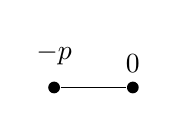
\begin{tikzpicture}[every node/.style={circle,fill=black,minimum width=1.5pt,inner sep=1.5pt}]
            \node[label={$-p$}] (A) at (0,0) {};
            \node[label={$0$}] (B) at (1,0) {};
            \draw (A) -- (B);
        \end{tikzpicture}
        \implies
        \begin{aligned}
            a_0 &= -1 & r_0 &= p \\
            a_1 &= 1 & r_1 &= 0
        \end{aligned}
    \end{equation*}
    $\mathbb{T}^1$ acts on $\mathbb{C}^2$ by $\lambda \cdot (z_1, z_2) = (\lambda z_1, \lambda z_2)$. $\pi=(-1,1)$ and $\iota=(1,1)^T$.
    The moment map $\iota^* \circ \mu : \mathbb{C}^2 \to (\mathfrak{t}^1)^*$ is given by
    \begin{equation*}
        \iota^*(\mu(z_1, z_2)) = \iota^*(-\pi|z_1|^2+p, -\pi|z_2|^2) = -\pi(|z_1|^2+|z_2|^2) + p.
    \end{equation*}
    Thus, $Z = (\iota^* \circ \mu)^{-1}(0) = (\iota^* \circ \mu_\textnormal{std})^{-1}(-p) = \{ z \in \mathbb{C}^2 \mid |z|^2 = p/\pi \}$. Hence $Z\simeq \mathbb{C}^2 / \mathbb{R}_{>0}$, $Z/\mathbb{T}^1 \cong \mathbb{P}^1$.

    For $\mathbb{P}^n$, consider the polytope
    \begin{equation*}
        \mathrm{conv}(\{ 0, e_1, \dots, e_n \})
        \implies
        \begin{aligned}
            a_0 &= (-1, \dots, -1) & r_0 &= p \in \mathbb{Z}_{>0} \\
            a_i &= e_i & r_i &= 0 \quad \forall 1 \leq i \leq n
        \end{aligned}
    \end{equation*}
    $\iota=(1,\dots ,1)^T$.
    Similarly, $\iota^* \circ \mu : \mathbb{C}^3 \to (\mathfrak{t}^1)^*$ is given by
    $\iota^*(\mu(z_0, \dots, z_n)) = -\pi(|z_0|^2+\cdots+|z_n|^2) + p$.
    $Z = (\iota^* \circ \mu)^{-1}(0) = \{ z \in \mathbb{C}^{n+1} \mid |z|^2 = p/\pi \}=\mathbb{C}^{n+1} / \mathbb{R}_{>0}/\mathbb{T}^1 \cong \mathbb{P}^n$.
\end{example}

\subsection{Equivalent Definition as GIT Quotient}

\label{sec:symplectic_reduction_as_git}

Write $G=(\mathbb{C}^\times )^k$, let character $\chi:G\rightarrow \mathbb{C}^\times $.
Let $L_{\chi^r}$ to be the linearized line bundle with character $\chi$, i.e. the sheaf of sections of $\mathbb{C}^n\times \mathbb{C}$ with $G$ action $g(p,t)=(g\cdot p,\chi(g)t)$.
Define the GIT quotient
\[
  \mathbb{C}^n\GIT_\chi:=\textnormal{Proj}\bigoplus _{r=0}^{\infty }\HH^0(\mathbb{C}^n,L_{\chi^r})^G=\textnormal{Proj}\bigoplus _{r=0}^{\infty }\CB{f\in \mathbb{C}[x_i]\mid f(g\cdot p)=\chi(g)^rf(p)\ \forall\ g\in G}.
\]
The Proj construction is defined on graded ring $S=\bigoplus _{n=0}^{\infty }S_n$ where $S_nS_m=S_{n+m}$. Let $S_+=\bigoplus _{n>0}S_n$. We denote $\textnormal{Proj}S\subseteq \textnormal{Spec}S$ to be the set of homogeous prime ideal $\mathfrak{p}$ s.t. $S_+\not\subseteq \mathfrak{p}$. Here, $\chi$ gives the grading on $\mathbb{C}[x_i]$ to talk about homogenousity.

\begin{example}[exp:GIT_P1_Proj]{}
  Consider the diagonal action $\mathbb{C}^*$ acting on $\mathbb{C}^2$. Let $\chi:G\rightarrow \mathbb{C}^\times$ be the identity, giving the standing grading on $S=\mathbb{C}[\mathbb{C}^2]=\mathbb{C}[x,y]$. Points in $\textnormal{Spec}S$: 
  \begin{itemize}
    \item $(0)$ is in $\Proj S$.
    \item Closed points are $(x-a,y-b)$. Homogenous implies $a=b=0$, yet $(x,y)=S_+$ is not in $\Proj S$.
    \item Irreducible homogenous prime ideals are $(ax+by)$, giving a $\mathbb{P}^1$ family of points in $\Proj S$.
  \end{itemize}
  The closed points in $\Proj S$ should then be thought of as maximal ideal in $\Proj S$, which corresponding to lines $k(ax+by)$ in $\Spec S$.

  Note that changing $\chi$ will be changing the grading, and hence $\Proj S$. A degenerate case is $\chi:(g)\mapsto 1$. The only invariant functions are constant functions. Hence $\Proj S=\Spec \mathbb{C}$ is a point.
\end{example}

A geometric way to understand GIT is by stability.
\begin{definition}[def:]{}
  Fix $G\subseteq (\mathbb{C}^\times )^n$ and character $\chi$ with linearized line bundle $L_\chi$. $p\in \mathbb{C}^n$ is
  \begin{itemize}
    \item semistable if there are $r>0$, $f\in \HH^0(\mathbb{C}^n,L_\chi^r)^G$ s.t. $f(p)\neq 0$,
    \item stable if semistable and $G_p$ is finite with $G$-orbits closed in $\mathbb{C}^n_f=\CB{p\in \mathbb{C}^n\mid f(p)\neq 0}$.
    \item unstable if not semistable.
  \end{itemize}
  Denote $(\mathbb{C}^n)^{\chi-\sstab}$ and $(\mathbb{C}^n)^{\chi-\stab}$ to be the set of semistable points and stable points respectively.
\end{definition}
The reason why it is geometric is because of the following theorem:
\begin{theorem}[thm:]{}
  Let $G\subseteq (\mathbb{C}^\times )^n$.
  $\mathbb{C}^n\GIT_\chi G=(\mathbb{C}^n)^{\chi-\sstab}\GIT G:=\Spec(\mathbb{C}[(\mathbb{C}^n)^{\chi-\sstab}]^G)$.
\end{theorem}

\begin{example}[exp:]{}
  Back to \Cref{exp:GIT_P1_Proj},  for $\chi:G\rightarrow \mathbb{C}^\times $ be the identity, every points $p$ except $(0,0)$ exists a homogeous function $f:(x,y)\mapsto x+y$ and $r=1$ that does not vanish at $p$.
\end{example}
\missing{Cover by open sets}


\missing{Frances Kirwan's thesis}
%http://www.cms.zju.edu.cn/UploadFiles/AttachFiles/201096185821505.pdf

\section{Hypertoric Varieties}
Hypertoric varieties is defined similar to the symplectic reduction construction for toric varieties $\mathbb{C}^n\GIT T_\mathbb{R}^k$. However, the fundamental building block changed to complex torus $T=\mathbb{C}^*$ acting on $T^*\mathbb{C}$ instead of $T_\mathbb{R}$ acting on $\mathbb{C}$; we consider general hyperplane arrangement instead of those arise from polytope; and the $(\mathbb{C}^*)^k$ action on $\mu^{-1}(0)$ may no longer be free. First, the moment map.
\begin{example}[exp:]{$(\mathbb{C^*})^n\acton T^*\mathbb{C}^n$}
  The $D=(\mathbb{C}^*)^n$-action on $T^*\mathbb{C}^n$ is given by $(t_iz_i,t^{-1}w_i)_{i=1}^{n}$.
  There is a canonical complex symplec form on $T^*\mathbb{C}^n$ by $\omega=\sum_{i}^{}dz_i\wedge dw_i$. Let $X_i\in \mathfrak{d}^n$ be a standard basis,
  \begin{alignat*}{1}
    (\ind{X_i})_z&=\frac{d}{dt}[e^{t_i}z_i,e^{-t_i}w_i]_{t=0}=(z_i\frac{\partial }{\partial z_i},-w_i\frac{\partial }{\partial w_i}),\\
    \iota_{\ind{X_i}}\omega&= (\sum_{}^{}dz_i\wedge dw_i)(z_i\partial/\partial z_i - w_i\partial/\partial w_i)=\sum z_idw_i + w_idz_i
  \end{alignat*}
  Thus, $\intd{\ind{X_i}}\omega = d(z_idw_i+w_idz_i) = d(z_iw_i)$. Hence $\mu(z_1,w_1,\dots ,z_n,w_n)=\sum_{}^{}z_iw_i$ is a moment map.
\end{example}

Given a short exact sequence of complex tori
\begin{equation*}
    \begin{tikzcd}
        1 \arrow[r] & G \arrow[r, "\iota"] & D \arrow[r, "\pi"] & T \arrow[r] & 1
    \end{tikzcd}
\end{equation*}
with $ D \cong (\mathbb{C}^\times)^n $, we consider
\begin{enumerate}
    \item the $G$-action on $T^*\mathbb{C}^n$ by $ g \cdot (z, w) = (\iota(g)_iz_i, \iota(g)_i^{-1}w_i)_{i=1}^n $, and
    \item the moment map $ \mu : T^*\mathbb{C}^n \to \mathfrak{g}^* $ for the $G$-action given by $ (z, w) \mapsto \iota^*((z_iw_i)_{i=1}^n) $.
\end{enumerate}
Similar to above, $\iota:G\rightarrow D$ and a choice of $ \lambda \in \mathfrak{g}^* $ define the symplectic reduction of $T^*\mathbb{C}^n$ by $G$ as the quotient $\mu^{-1}(\lambda)$ by $G$. However, $G$ may not act freely on $\mu^{-1}(\lambda)$, and hence we need further pick a character $ \chi : G \to \mathbb{C}^\times $ and define the hypertoric variety to be the GIT quotient
\begin{equation*}
  \mathcal{M}_{\chi, \lambda} = T^*\mathbb{C}^n \HQ[\chi, \lambda] G = \mu^{-1}(\lambda) \GIT[\chi] G:=\textnormal{Proj}\bigoplus _{r=0}^{\infty }\CB{f\in \textnormal{Fun}(\mu^{-1}(\lambda))\mid f(g\cdot x)=\chi(g)^rf(x)\ \forall\ g}.
\end{equation*}
\noskipline
\begin{remark}
  Recall in \Cref{sec:symplectic_reduction_as_git} that we can realize the GIT quotient of complex torus as the symplectic reduction of the real torus. One can alternatively define hypertoric varieties as the hyperkahler quotient of $T^*\mathbb{C}^n$ by $G_\mathbb{R}$ at the value $(\chi,\textnormal{Re }\lambda,\textnormal{Im }\lambda)$, which is naturally diffeomorphic to $\MM_{\chi,\lambda}$.
\end{remark}

\begin{example}{$\mathbb{C}^\times \acton T^*\mathbb{C}^{n+1}$}
  Let $G=\mathbb{C}^\times$ and $D=(\mathbb{C}^\times )^{n+1}$ with $\iota:G\rightarrow D$ given by the diagonal map.
    The action $\mathbb{C}^\times$ on $T^*\mathbb{C}^{n+1}$ is given by $\lambda \cdot (z, w) = (\lambda z, \lambda^{-1} w)$. We have
    \begin{align*}
        \mu^{-1}(0) &= \{ (z, w) \in T^*\mathbb{C}^{n+1} \mid z_0w_0 = z_1w_1 + \cdots + z_nw_n \}.
    \end{align*}
    Let $\chi : \lambda \mapsto \lambda^p$ be the character of $G$.
    We now establish the stability of the action. Note that for all $r>0$, the only function $f$ on $T^*\mathbb{C}^{n+1}$ satisfying $f(0, \lambda^{-1}w)=\lambda^{rp} \, f(0, w)$ for all $\lambda \in \mathbb{C}^\times$ is $f=0$. Thus, $(0, w) \notin (T^*\mathbb{C}^{n+1})^\sstab$. Conversely, suppose $z \neq 0$. Then, we may pick $f(z, w) = z^p$, which satisfies the equation $f(\lambda z, \lambda^{-1}w) = \lambda^p \, f(z, w)$ for all $\lambda \in \mathbb{C}^\times$. Thus, $(z, w)$ is semistable. Moreover, the orbit $T \cdot (z, w)$ is closed in the non-vanishing locus of $f$, and the orbit is clearly of dimension 1. Thus, $(z, w)$ is stable. In conclusion, we have
    \begin{enumerate}
        \item $(T^*\mathbb{C}^{n+1})^\sstab = (T^*\mathbb{C}^{n+1})^\stab = T^*\mathbb{C}^{n+1} \setminus \{ z=0 \}$, and
        \item $\mu^{-1}(0)^\sstab = \mu^{-1}(0)^\stab = \{ (z, w) \mid z_0w_0 = z_1w_1 + \cdots + z_nw_n, z \neq 0 \}$.
    \end{enumerate}

    After taking quotients, we have the following diagram.
    \begin{equation*}
        \begin{tikzcd}
            \mu^{-1}(0)^\stab \arrow[d, hookrightarrow] \arrow[r] & \mu^{-1}(0) \GIT[\chi] \mathbb{C}^\times \arrow[dd, dashed, "\pi"] \\
            (T^*\mathbb{C}^{n+1})^\stab \arrow[d] & {} \\
            \mathbb{C}^{n+1} \setminus \{ 0 \} \arrow[r] & \mathbb{C}^{n+1} \GIT[\chi] \mathbb{C}^\times = \mathbb{P}^n
        \end{tikzcd}
    \end{equation*}
    Note that the composite on the LHS is $\mathbb{C}^\times$-equivariant, thus it descents to the dashed arrow $\pi$. We claim that $T^*\mathbb{C}^{n+1} \HQ[\chi] \mathbb{C}^\times = T^*\mathbb{P}^n$. Note that
    \begin{align*}
        T^*\mathbb{C}^{n+1} \HQ[\chi] \mathbb{C}^\times = \mu^{-1}(0)^\stab / \mathbb{C}^\times = (T^*\mathbb{C}^{n+1} \setminus \{ 0 \}) \GIT \mathbb{C}^\times && \text{since} && \mu^{-1}(0)^\stab = \left(\mu|_{T^*(\mathbb{C}^{n+1} \setminus \{ 0 \})}\right)^{-1}(0).
    \end{align*}
    The claim then follows from Proposition~\ref{prop:cot red} by setting $M = \mathbb{C}^{n+1} \setminus \{ 0 \}$ and $G = \mathbb{C}^\times$.
\end{example}

\begin{proposition}[prop:cot red]{}
  Let $M$ be a smooth manifold with a free and proper $G$-action. This induces a Hamiltonian $G$-action on $T^*M$ with moment map $\mu : T^*M \to \mathfrak{g}^*$. Then, $(T^*M) \GIT G \cong T^*(M/G)$.
  \begin{proof}
    As $G \acton M$ is free and proper, $M/G$ is a smooth manifold. Let $\pi : T^*M \to M$ be the projection and consider the induced action $G$ on $T^*M$. 
    Define the tautological form $\theta \in \df^1(T^*M)$ by
        \begin{equation*}
            \theta_{(p, \alpha)} = d\pi_{(p, \alpha)}^*(\alpha) \quad \text{ i.e.} \quad \theta_{(p, \alpha)}(v) = \alpha(d\pi_{(p, \alpha)}(v))
        \end{equation*}
        for all $p \in M$, $\alpha \in T_p^*M$, $v \in T_{(p, \alpha)}(T^*M)$. Define $\omega = -d\theta$. Then, $(T^*M, \omega)$ is a symplectic manifold. Let $(p_1, \dots, p_n, \alpha^1, \dots, \alpha^n)$ be a local coordinate of $U \subseteq T^*M$. Then, $\theta|_U = \sum_i \alpha^i \, dp_i$ and $\omega|_U = \sum_i d\alpha^i \wedge dp_i$. We claim that the action $G$ on $T^*M$ given by $g\cdot (p,\alpha)=(g\cdot p,d(g^{-1})^*_p(\alpha))$ is hamiltonian with a canonical choice of moment map given by $\mu(p,\alpha)(X)=\alpha(\ind{X_p})$ for all $X \in \mathfrak{g}$.

    Note that we have the following isomorphisms, where $\perp$ denotes the annihilator.
    \begin{align*}
      T_{[p]}(M/G) \cong T_pM / T_p(G \cdot p) && T_{[p]}^*(M/G) \cong T_p(G \cdot p)^\perp \subseteq T_p^*M
    \end{align*}
    Let $\pi : TM \to T(M/G)$ be the projection. Note that $\ker(\pi_p) \cong T_p(G \cdot p)$. Using the fact that $G$ act on $M$ is free, we can show that $\ker(\pi_p) = \{ v \in T_pM \mid \pi(p, v) = 0 \} = \{ \ind{X}_p \mid X \in \mathfrak{g} \} \cong \mathfrak{g}$ for all $p \in M$.

    Let $\tau : (T^*M) \GIT G \to M/G$ be the map induced by the $G$-equivariant map $\mu^{-1}(0) \to M$. Then, $\tau$ is surjective since for all $p \in M$, $(p, 0) \in \mu^{-1}(0)$. Let $p \in M$. Since $G$ acts on $M$ freely, the fiber $\tau^{-1}([p])$ has the following description.
    \begin{align*}
      \tau^{-1}([p]) &= \{ [p, \alpha] \mid (p, \alpha) \in \mu^{-1}(0) \} \\
                     &\cong \{ \alpha \in T_p^*M \mid \mu(p, \alpha) = 0 \} = \{ \alpha \in T_p^*M \mid \alpha(\ind{X}_p) = 0 \quad \forall X \in \mathfrak{g} \} \\
                     &= \{ \ind{X}_p \mid X \in \mathfrak{g} \}^\perp = \ker(\pi_p)^\perp \cong T_p(G \cdot p)^\perp = T_p^*M
    \end{align*}
    This gives the required isomorphism $(T^*M) \GIT G \cong T^*(M/G)$.
  \end{proof}
\end{proposition}

\section{Combinatorial Description}

\subsection{Hyperplane Arrangement}

There is a remaining $T$-action on the quotient with a moment map $ \nu : \mathcal{M}_{\chi, \lambda} \to \mathfrak{t}^* $. We will always set $\lambda=0$. In this case, the above data can be assembled into a hyperplane arrangement with $n$ hyperplanes in the affine subspace $ (\iota_{\mathbb{R}}^*)^{-1}(\chi) = \{ x \in \mathfrak{d}_{\mathbb{R}}^* \mid \iota_{\Gamma}^*(x) = \chi \} $ of $\mathfrak{d}_{\mathbb{R}}^*$, where the $i$-th hyperplane is the intersection of $(\iota_{\mathbb{R}}^*)^{-1}(\chi)$ with the $i$-th coordinate hyperplane in $\mathfrak{d}_{\mathbb{R}}^*$. Conventionally, one choose a lift $\theta$ of $\chi$ along $\iota_\mathbb{R}^*$, allowing us to identify the affine subspace $(\iota_{\mathbb{R}}^*)^{-1}(\chi)$ with $\mathfrak{t}_\mathbb{R}^*$. This gives a hyperplane arrangement
\begin{equation*}
    \mathcal{A}_\chi = \{ H_i = \{ x \in \mathfrak{t}_{\mathbb{R}}^* \mid \pi^*(x)_i = \theta_i \} \}_{i=1}^n.
\end{equation*}
Different choices of lifts give the same hyperplane arrangement up to translations.

\subsection{Graph}

<++>

\subsection{GIT}
\subsection{Stability Condition}
For both $\theta$ and $\lambda$
\section{GKM Graph of Hypertoric}
\subsection{Fix Points}
\subsection{Connecting P1}
How $\theta$ effects the splitting of $S^+$
\subsection{Matroid Polytope}
\subsection{Equivariant Cohomology of Hypertoric}
\section{Line Bundles on Hypertoric}
\section{Steinberg Correspondences}
\subsection{Primitive Coroots and Hyperplane}
\subsection{Steinberg Varieties}

\section{Comparing Stability Condition with Quiver Varieties}
\section{Arxiv}

\begin{example}{$\mathbb{T}^n \acton T^*\mathbb{C}^{n+1}$}
    Consider the hyperplane arrangement in $\mathbb{R}$ given by the following data.
    \begin{equation*}
        \begin{aligned}
            a_i &= 1 & r_i &= i & \forall 0 \leq i \leq n
        \end{aligned}
    \end{equation*}
    The induced short exact sequences of tori are as follows.
    \begin{equation*}
        \begin{tikzcd}[row sep=0ex]
            0 \arrow[r] & \mathfrak{t}^n \arrow[r, "\iota"] & \mathfrak{t}^{n+1} \arrow[r, "\pi"] & \mathfrak{t}^1 \arrow[r] & 0 \\
            {} & (x_1, \dots, x_n) \arrow[r, maps to] & (-\sum_i x_i, x_1, \dots, x_n) & {} & {} \\
            0 & (\mathfrak{t}^n)^* \arrow[l] & (\mathfrak{t}^{n+1})^* \arrow[l, "\iota^*"'] & (\mathfrak{t}^1)^* \arrow[l, "\pi^*"'] & 0 \arrow[l] \\
            {} & (x_1-x_0, \dots, x_n-x_0) & (x_0, \dots, x_n) \arrow[l, maps to] & {} & {}
        \end{tikzcd}
    \end{equation*}
    The action $\mathbb{T}^n \acton T^*\mathbb{C}^{n+1}$ is as follows.
    \begin{equation*}
        (\lambda_1, \dots, \lambda_n) \cdot
        \begin{bmatrix}
            z \\
            w
        \end{bmatrix}
        =
        \begin{bmatrix}
            \lambda_1^{-1} \dots \lambda_n^{-1} z_0 & \lambda_1z_1 & \cdots & \lambda_nz_n \\
            \lambda_1 \dots \lambda_n w_0 & \lambda_1^{-1}w_1 & \cdots & \lambda_n^{-1}w_n
        \end{bmatrix}
    \end{equation*}
    The complex moment map $\mu : T^*\mathbb{C}^{n+1} \to (\mathfrak{t}^n)^*$ and its zero locus are as follows.
    \begin{align*}
        \mu(z, w) &= (z_1w_1-z_0w_0, \dots, z_nw_n-z_0w_0) \\
        \mu^{-1}(0) &= \{ (z, w) \in T^*\mathbb{C}^{n+1} \mid z_0w_0 = z_1w_1 = \cdots = z_nw_n \}
    \end{align*}
    The character is given by $\alpha : (\lambda_1, \dots, \lambda_n) \mapsto \lambda_1 \lambda_2^2 \cdots \lambda_n^n$.

    Define $U_i = \{ (z, w) \in \mu^{-1}(0) \mid w_0, \dots, w_{i-1}, z_{i+1}, \dots, z_n \neq 0 \}$ for all $0 \leq i \leq n$. We claim that $\mu^{-1}(0)^\sstab = U_0 \cup \cdots \cup U_n$. Indeed, in $U_i$, we can pick the polynomial
    \begin{align*}
        f(z, w) = w_0^i w_1^{i-1} \cdots w_{i-1} z_{i+1} z_{i+2}^2 \cdots z_n^{n-i} && \text{satisfying} && f(\lambda \cdot z, \lambda^{-1} \cdot w) = \lambda_1 \lambda_2^2 \cdots \lambda_n^n \, f(z, w).
    \end{align*}
    Note that $\mu^{-1}(0) \setminus (U_0 \cup \cdots \cup U_n) = \{ (z, w) \in \mu^{-1}(0) \mid w_j = z_i = 0 \text{ for some } 0 \leq j < i \leq n \}$. Now fix $0 \leq j < i \leq n$ and suppose $w_j = z_i = 0$. Suppose we have a polynomial $f$ satisfying $f(\lambda \cdot z, \lambda^{-1} \cdot w) = \lambda_1^r \lambda_2^{2r} \cdots \lambda_n^{nr} \, f(z, w)$ for some $r>0$. For a positive power of $\lambda_i$ to appear in the RHS, either $f$ has a factor of $z_i$, or $f$ has no factor of $z_i$ but a factor of $w_0^{ir}$. The former case causes $f(z, w)=0$. In the latter case, $f$ must also have a factor of $w_j$ to lower the power of $\lambda_j$, causing $f(z, w)=0$ again. We conclude that $(z, w)$ is indeed not semistable.

    Then, we claim that $\mu^{-1}(0)^\sstab = \mu^{-1}(0)^\stab$. Let $(z, w) \in U_i$. As $w_0, \dots, w_{i-1}, z_{i+1}, \dots, z_n \neq 0$, it is clear that the orbit is of dimension $n$. To show the closedness of the orbit $\mathbb{T}^n \cdot (z, w)$, it suffices to show that for all non-trivial one parameter subgroup. Let $\varphi : \mathbb{C}^\times \to \mathbb{T}^n$ be given by $(\varphi_1, \dots, \varphi_n) \in \mathbb{Z} \setminus \{ 0 \}$. Then, there exists $1 \leq j \leq n$ such that $\varphi_j \neq 0$. Then, as $\lambda \to 0/\infty$, $\lambda^{-1} \cdot w_j \to 0/\infty$ if $j<i$ and $\lambda \cdot z_j \to 0/\infty$ if $j>i$, so that the limit is outside $\mu^{-1}(0)^\sstab$. It remains to consider the case where $\varphi_j=0$ for all $j\neq i$. In this case, when $\lambda \to 0/\infty$, $w_0 \to 0/\infty$, which makes the limit outside $\mu^{-1}(0)^\sstab$ again. We conclude that the orbit is closed. Hence, $\mu^{-1}(0)^\sstab = \mu^{-1}(0)^\stab$.

    With the above arguments, we showed that $T^*\mathbb{C}^{n+1} \HQ[\alpha] \mathbb{T}^n = (U_0 \cup \cdots \cup U_n) / \mathbb{T}^n$. It is clear that $U_i/\mathbb{T}^n \cong T^*\mathbb{C}$ with projections given by
    \begin{align*}
        U_i \to T^*\mathbb{C} && (z, w) \mapsto (w_0^{-1} \cdots w_{i-1}^{-1} z_i \cdots z_n, w_0 \cdots w_i z_{i+1}^{-1} \cdots z_n^{-1}).
    \end{align*}
    Define $V_i = T^*\mathbb{C}$ for all $0 \leq i \leq n$, thought of as $U_i/\mathbb{T}^n$. Then, $T^*\mathbb{C}^{n+1} \HQ[\alpha] \mathbb{T}^n$ is the union of the $V_i$'s glued together
    \begin{equation*}
        \begin{tikzcd}[row sep=tiny, column sep=small, /tikz/column 1/.append style={anchor=base east}]
            {} & V_j & V_i \\
            \text{along} & \{ w \neq 0 \} \arrow[u, phantom, "\subseteq" rotate=90] \arrow[r, phantom, "\cong"] & \{ z \neq 0 \} \arrow[u, phantom, "\subseteq" rotate=90] \\
            \text{using the isomorphisms} & (z, w) \arrow[r, maps to] & (z^{j-i+1}w^{j-i}, z^{i-j}w^{i-j+1}) \\[-1ex]
            \text{and} & (z^{i-j+1}w^{i-j}, z^{j-i}w^{j-i+1}) & (z, w) \arrow[l, maps to]
        \end{tikzcd}
    \end{equation*}
    for all $0 \leq j < i \leq n$.
\end{example}

\appendix


%\bibliographystyle{alpha}
%\bibliography{ref}

\end{document}
